\documentclass[letterpaper,10pt]{article}

\usepackage{enumitem}
\usepackage{titling}
\usepackage{listings,listings-rust}
\usepackage{url}
\usepackage{soul}
\usepackage{hyperref}
\usepackage{setspace}
\usepackage{subfig}
\usepackage{sectsty}
\usepackage{pdfpages}
\usepackage{colortbl}
\usepackage{multirow}
\usepackage{multicol}
\usepackage{relsize}
\usepackage{amsmath}
\usepackage{wasysym}
\usepackage{fancyvrb}
\usepackage[yyyymmdd]{datetime}
\usepackage{amsmath,amssymb,amsthm,graphicx,xspace}
\usepackage[titlenotnumbered,noend,noline]{algorithm2e}
\usepackage[compact]{titlesec}
\usepackage{XCharter}
\usepackage[T1]{fontenc}
\usepackage[scaled]{beramono}
\usepackage[normalem]{ulem}
\usepackage{booktabs}
\usepackage{tikz}
\usetikzlibrary{arrows.meta,automata,shapes,trees,matrix,chains,scopes,positioning,calc,decorations.pathreplacing}
\tikzstyle{block} = [rectangle, draw, fill=blue!20, 
    text width=2.5em, text centered, rounded corners, minimum height=2em]
\tikzstyle{bw} = [rectangle, draw, fill=blue!20, 
    text width=4em, text centered, rounded corners, minimum height=2em]

\definecolor{namerow}{cmyk}{.40,.40,.40,.40}
\definecolor{namecol}{cmyk}{.40,.40,.40,.40}
\renewcommand{\dateseparator}{-}

\let\LaTeXtitle\title
\renewcommand{\title}[1]{\LaTeXtitle{\textsf{#1}}}

\lstset{basicstyle=\footnotesize\ttfamily,breaklines=true}

\newcommand{\CPP}{C\nolinebreak\hspace{-.05em}\raisebox{.4ex}{\tiny\bf +}\nolinebreak\hspace{-.10em}\raisebox{.4ex}{\tiny\bf +}}
\def\CPP{{C\nolinebreak[4]\hspace{-.05em}\raisebox{.4ex}{\tiny\bf ++}}}

\newcommand{\handout}[5]{
  \noindent
  \begin{center}
  \framebox{
    \vbox{
      \hbox to 5.78in { {\bf ECE459: Programming for Performance } \hfill #2 }
      \vspace{4mm}
      \hbox to 5.78in { {\Large \hfill #4  \hfill} }
      \vspace{2mm}
      \hbox to 5.78in { {\em #3 \hfill \today} }
    }
  }
  \end{center}
  \vspace*{4mm}
}

\newcommand{\lecture}[3]{\handout{#1}{#2}{#3}{Lecture#1}}
\newcommand{\tuple}[1]{\ensuremath{\left\langle #1 \right\rangle}\xspace}

\addtolength{\oddsidemargin}{-1.000in}
\addtolength{\evensidemargin}{-0.500in}
\addtolength{\textwidth}{2.0in}
\addtolength{\topmargin}{-1.000in}
\addtolength{\textheight}{1.75in}
\addtolength{\parskip}{\baselineskip}
\setlength{\parindent}{0in}
\renewcommand{\baselinestretch}{1.5}
\newcommand{\term}{Winter 2020}

\singlespace


\begin{document}

\lecture{5 --- Asynchronous I/O}{\term}{Patrick Lam}

\section*{Asynchronous/non-blocking I/O}

\begin{center}
  \fbox{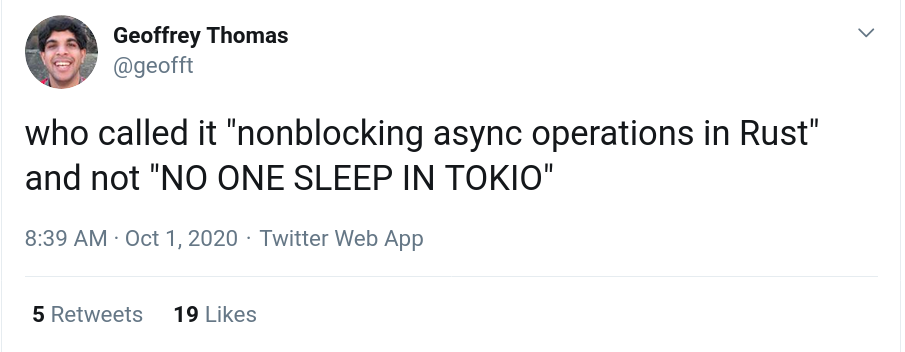
\includegraphics[width=.7\textwidth]{images/L05-tokio.png}}
\end{center}

To motivate the need for non-blocking I/O, consider some standard I/O code:

\begin{lstlisting}[language=Rust]
fn main() -> io::Result<()> {
  let mut file = File::open("hello.txt")?;
  let mut s = String::new();
  file.read_to_string(&mut s)?;
  Ok(()) 
}
\end{lstlisting}
(The ? operator ``for easier error handling'' is an alternative to
\texttt{try!} and \texttt{unwrap}.)

This isn't very performant. The problem is that the {\tt read} call will
{\em block}. So, your program doesn't get to use the zillions of CPU cycles that
are happening while the I/O operation is occurring.

\paragraph{As seen previously: threads.} Threads can be fine if
you have some other code running to do work---for instance, other threads
do a good job mitigating the I/O latency, perhaps doing I/O themselves.
But maybe you would rather not use threads. Why not?
\begin{itemize}[noitemsep,topsep=-1em]
\item potential race conditions;
\item overhead due to per-thread stacks; or
\item limitations due to maximum numbers of threads.
\end{itemize}

\subsection*{Doing non-blocking I/O}
We're going to focus on low-level I/O from sockets in this part of the lecture,
using the \texttt{mio}\footnote{\url{https://tokio-rs.github.io/mio/doc/mio/}} library from \texttt{tokio}. Async file I/O is
also possible via \texttt{tokio::fs} and the ideas will carry over.
One might often want to wrap the low-level I/O using higher-level
abstractions, and the larger project \texttt{tokio.rs} is one way of
doing that.

Fundamentally,
there are two ways to find out whether I/O is ready to be queried:
polling (under UNIX, implemented via {\tt select}, {\tt poll}, and
{\tt epoll}) and interrupts (under UNIX, signals). \texttt{mio}
supports polling-based approaches and abstracts across Linux (via
epoll), Windows (via IOCP), and BSDs including MacOS (via kqueue).

The key idea is to give {\tt mio} a bunch of event sources and
wait for events to happen. In particular:
     \begin{itemize}[noitemsep,topsep=-1em]
       \item create a \texttt{Poll} instance;
       \item populate it with event sources e.g. \texttt{TCPListener}s; and,
       \item wait for events in an event loop ({\tt Poll::poll()}).
     \end{itemize}
Let's run through these steps in order, following \url{https://docs.rs/mio/0.7.0/mio/guide/index.html}:

\paragraph{Creating a {\tt Poll} instance.} Just use the API:
    \begin{lstlisting}[language=Rust]
let poll = Poll::new()?;
let events = Events::with_capacity(128);
    \end{lstlisting}
We're going to proactively create \texttt{events}; this data structure is used by
\texttt{Poll::poll} to stash the relevant \texttt{Event} objects.

The \texttt{poll} object keeps track of event sources and,
on request, pulls the events from the sources and puts them
into the argument to \texttt{Poll::poll()}.

\paragraph{Populating the {\tt Poll} instance.} The docs refer
to this as ``registering event source''. On all platforms this can be
a socket (or lower-level networking source); on UNIX it can be also be
a file descriptor.

\begin{lstlisting}[language=Rust]
let mut listener = TcpListener::bind(address)?;
const SERVER: Token = Token(0);
poll.registry().register(&mut listener, SERVER, Interest::READABLE)?;
\end{lstlisting}

The payload is the \texttt{register} call. Parameters, going right-to-left:
\begin{itemize}[noitemsep]
\item You're telling it to check for 
when the \texttt{listener} indicates that something is available to read
(``\texttt{READABLE}'').
\item The \texttt{SERVER} parameter
is a note-to-self saying that events indicated with this particular
\texttt{listener} should be flagged with the \texttt{SERVER} token.
(Otherwise, if you register multiple listeners, you will have a bunch
of events and not know which listener they came from.)
\item Finally, the provided
\texttt{listener} watches for connections on \texttt{address} (not provided here,
but can be a \texttt{host:port} string).
\end{itemize}

\paragraph{Waiting on an {\tt Poll} instance.} Having completed
the setup, we're ready to wait for events on any registered listener.
    \begin{lstlisting}[language=Rust]
loop {
    poll.poll(&mut events, Some(Duration::from_millis(100)))?;

    for event in events.iter() {
        match event.token() {
            SERVER => loop {
                match listener.accept() {
                    Ok((connection, address)) => {
                        println!("Got a connection from: {}", address);
                    },
                    Err(ref err) if would_block(err) => break,
                    Err(err) => return Err(err),
                }
            }
        }
    }
}

fn would_block(err: &io::Error) -> bool {
    err.kind() == io::ErrorKind::WouldBlock
}    \end{lstlisting}
As foreshadowed, \texttt{poll.poll} will populate \texttt{events}, and
waits for at most 100 milliseconds. A timeout of \texttt{None} will block
until an event occurs.

Note the use of the \texttt{SERVER} token when processing the event.
If there were multiple listeners, you would give them each a different
token. Each event may correspond to one or more connections.

You can find the complete example here:
\begin{center}
\url{https://docs.rs/mio/0.7.0/mio/struct.Poll.html}
\end{center}

\section*{Network Programming}
If all you want to do is request a web page in Rust, use
the \texttt{reqwest} library (\url{https://docs.rs/reqwest/0.10.8/reqwest/}),
which has both blocking and non-blocking interfaces. Here's the
non-blocking interface:
    \begin{lstlisting}[language=Rust]
let body = reqwest::get("https://www.rust-lang.org")
    .await?
    .text()
    .await?;

println!("body = {:?}", body);
\end{lstlisting}
(If you are doing multiple requests,
you should create your own \texttt{Client} and \texttt{get} from it instead of
\texttt{reqwest::get}).

\paragraph{Back to the Futures.}
The use of \texttt{await} is a bit tricky. If you took CS~343
(for instance, because you are an SE student), then you will have seen
the concept. Otherwise I'll briefly explain futures from first principles.
You can find Rust documentation on them here:
\begin{center}
\url{https://rust-lang.github.io/async-book/01_getting_started/04_async_await_primer.html}
\end{center}

The \texttt{get} function returns a \emph{future}. What's that?  It's
an object that will, at some point in the future, return a second
object.

Here's an analogy. I go to Ziggy's Cycles and try to purchase a
bicycle. Since there's currently a pandemic going on in Canada as I
write this in September 2020, and bicycles are more popular than
usual, it's reasonable to expect that they might actually be out of
bicycles at the moment, and so they can't
give me a bicycle right away.  But they'll take my money and
specifications for a desired bicycle and give me a ticket (the
future). Some time later, I can trade in that ticket (await) for an
actual bicycle.

\paragraph{Plug-in Executors.}
There are many possible definitions of \texttt{async/await}, and the appropriate
one depends on your context. Rust allows you to specify a runtime
which defines the meaning of \texttt{async/await} for your program.

The simplest \texttt{await} just blocks and waits on the current
thread for the result to be ready. A Rust library
provides \texttt{futures::executor::block\_on} with that
simplest functionality.

\begin{lstlisting}[language=Rust]
use futures::executor::block_on;

async fn hello_world() {
  println!("hello");
}

fn main() {
  let future = hello_world();
  block_on(future);
}
\end{lstlisting}
Even that executor requires you to declare dependency \texttt{futures = "0.3"}
in Cargo.toml; Build with \texttt{cargo build} and run with \texttt{cargo run}. The full code is in the course repo under \texttt{live-coding/L05/block-on}.

\texttt{tokio} includes a more sophisticated executor as well; e.g. when
there are multiple active \texttt{await}s, \texttt{tokio} can multiplex them onto
different threads. You can specify the \texttt{tokio} executor (or others) with a
tag above {\tt main()} and by declaring \texttt{main()} to be \texttt{async},
instead of what we did above with explicitly calling \texttt{block\_on}.
There are other tags to choose other executors (e.g. \texttt{async\_std}).
\begin{lstlisting}[language=Rust]
#[tokio::main]
async fn main() {
    // do async stuff
}
\end{lstlisting}
You can read more about tokio here:
\begin{center}
\url{https://medium.com/@alistairisrael/demystifying-closures-futures-and-async-await-in-rust-part-3-async-await-9ed20eede7a4}
\end{center}

\subsection*{Using libcurl: easy}
libcurl is a C library for transferring files. It has Rust bindings and we'll
explain how to use those.

First we'll start with the easy interface. This is a synchronous interface
that uses callbacks. Here's some code from the Rust bindings documentation
(\url{https://docs.rs/curl/0.4.33/curl/}):

\begin{lstlisting}[language=Rust]
use std::io::{stdout, Write};

use curl::easy::Easy;

// Write the contents of rust-lang.org to stdout
let mut easy = Easy::new();
easy.url("https://www.rust-lang.org/").unwrap();
easy.write_function(|data| {
    stdout().write_all(data).unwrap();
    Ok(data.len())
}).unwrap();
easy.perform().unwrap();
\end{lstlisting}
Note that we provide a lambda as a callback function. This lambda is to be invoked
when the library receives data from the network (i.e. \texttt{write\_function()}).

In the body of the lambda, we simply write the received data to \texttt{stdout}
and return the number of bytes we processed (all of them, in this case).
Looking at the original libcurl documentation (\url{https://curl.haxx.se/libcurl/c/CURLOPT_WRITEFUNCTION.html}), you'll see how the Rust bindings
are a fairly straightforward translation.

We call \texttt{easy.perform()} to, well, perform the request, blocking until
it finishes, and using the callback to process the received data.

\subsection*{Using libcurl: multi}
The real reason we're talking about libcurl is the asynchronous multi interface;
network communication is a great example of asynchronous  I/O.
You can start a network request and move on to creating more without waiting for the results of the first one. For requests to different recipients, it certainly makes sense to do this.

The main tool here is the ``multi handle''---this is a structure that lets us have more than one curl easy handle. And rather than waiting, we can start them and then check on their progress. 

The structure for the new multi-handle type is \texttt{curl::multi::Multi} (instead of \texttt{curl::easy::Easy}) and it is initialized with the \texttt{new()} function. The multi functions may return a \texttt{MultiError} rather than the easy \texttt{Error}, and I don't know how to unify the error handling with ? here.

Once we have a multi handle, we can add easy objects---however many we need---to the multi handle. Creation of the easy object is the same as it is when being used alone---use \texttt{Easy::new()} to create it and set options on that handle. The documentation suggests that an \texttt{Easy2} might be better for use with multi handles. Then, we add the easy (or easy2) object to the multi handle with \texttt{add()} (or \texttt{add2()}). The \texttt{add()} or \texttt{add2()} functions return an actual easy handle.

Once we have finished putting all the easy handles into the multi handle, we can dispatch them all at once with \texttt{perform()}. This function returns, on success, the number of easy handles in that multi handle that are still running. If it's down to 0, then we know that they are all done. If it's nonzero it means that some of them are still in progress.

This does mean that we're going to call \texttt{perform()} more than once. Doing so doesn't restart or interfere with anything that was already in progress---it just gives us an update on the status of what's going on. We can check as often as we'd like, but the intention is of course to do something useful while the asynchronous I/O request(s) are going on. Otherwise, why not make it synchronous? 

Suppose we've run out of things to do though. What then? Well, we can wait, if we want, using \texttt{wait()}. This function will block the current thread until something happens (some event occurs).

The first parameter to \texttt{wait()} is an array of extra file descriptors you can wait on (but we will always want this to be \texttt{\&mut []} in this course). The second parameter is a maximum time to wait. The return value is the actual number of ``interesting'' events that occurred (interesting is the word used in the specifications, and what it means is mysterious). For a simple use case you can ignore most of the parameters and just wait for something to happen and go from there.

In the meantime though, the perform operations are happening, and so are whatever callbacks we have set up (if any). And as the I/O operation moves through its life cycle, the state of the easy handle is updated appropriately. Each easy handle has an associated status message as well as a return code.

Why both? Well---one is about what the status of the request is. The message could be, for example, ``done'', but does that mean finished with success or finished with an error? The second one tells us about that. We can allegedly ask about the status of the request using \texttt{messages()}, and we're really supposed to do that if we use \texttt{action()} (which we don't talk about) rather than \texttt{perform()} (which we do).

We pass \texttt{messages()} a callback which finds out what happened and makes sure all is well. This callback is an \texttt{FnMut} and hence allowed to mutate state. What we are looking for is that the callback's parameter \texttt{msg} has \texttt{result\_for} including \texttt{Some}---request completed. If not, this request is still in progress and we aren't ready to evaluate whether it was successful or not. If there are more handles to look at, we should go on to the next. If it is done, we should look at the result. If it is \texttt{Error} then there is an error. Else, everything succeeded.

When a handle has finished, you need to remove it from the multi handle. Remove the handle you got back from \texttt{add/2} with \texttt{remove/2}. You don't have to cleanup the easy handle because Rust.

Let's consider the following code example by Clemens Gruber~\cite{curlmulti}, which I've translated to Rust (mostly). This example puts together all the things we talked about in one compact code segment. Here, the callback prints the data to \texttt{stdout}.

\begin{lstlisting}[language=Rust]
const URLS:[&str; 4] = [
  "https://www.microsoft.com",
  "https://www.yahoo.com",
  "https://www.wikipedia.org",
  "https://slashdot.org" ];

use curl::Error;
use curl::easy::{Easy2, Handler, WriteError};
use curl::multi::{Easy2Handle, Multi};
use std::time::Duration;
use std::io::{stdout, Write};

struct Collector(Vec<u8>);
impl Handler for Collector {
    fn write(&mut self, data: &[u8]) -> Result<usize, WriteError> {
        self.0.extend_from_slice(data);
	stdout().write_all(data).unwrap();
        Ok(data.len())
    }
}

fn init(multi:&Multi, url:&str) -> Result<Easy2Handle<Collector>, Error> {
    let mut easy = Easy2::new(Collector(Vec::new()));
    easy.url(url)?;
    easy.verbose(false)?;
    Ok(multi.add2(easy).unwrap())
}

fn main() {
    let mut easys : Vec<Easy2Handle<Collector>> = Vec::new();
    let mut multi = Multi::new();
    
    multi.pipelining(true, true).unwrap();
    for u in URLS.iter() {
	easys.push(init(&multi, u).unwrap());
    }
    while multi.perform().unwrap() > 0 {
	// .messages() may have info for us here...
        multi.wait(&mut [], Duration::from_secs(30)).unwrap();
    }

    for eh in easys.drain(..) {
    	let mut handler_after:Easy2<Collector> = multi.remove2(eh).unwrap();
        println!("got response code {}", handler_after.response_code().unwrap());
    }
}
\end{lstlisting}

You may wonder about re-using an easy handle rather than removing and destroying it and making a new one. The official docs say that you can re-use one, but you have to remove it from the multi handle and then re-add it, presumably after having changed anything that you want to change about that handle. 

Because a handle could be replaced with another one (or the same one), you could have a situation where there are constantly handles in progress and you might never be at a situation where there are no messages left. And that is okay.

In this example all requests had the same callback, but of course you could have different callbacks for different easy handles if you wanted them to do different things.

How well does this scale? The developer claims that you can have multiple thousands of connections in a single multi handle\footnote{See this post from the mailing list: \url{https://curl.haxx.se/mail/lib-2011-11/0078.html}}. And 60k ought to be enough for anyone!

\paragraph{I enjoy pain!} You can use cURL with \texttt{select()} if you wish, although it comes with an anti-recommendation: I think you shouldn't do it. But you can if you want. In some ways, cURL does make things less painful because it does some of the grunt work for you. Don't do it. Please no.

\section*{Building Servers: Concurrent Socket I/O}

\paragraph{Your Choices.} The first two both use blocking I/O, while the second two use
non-blocking I/O~~\cite{gplus:concurrent}:
    \begin{itemize}
      \item Blocking I/O; 1 process per request.
      \item Blocking I/O; 1 thread per request.
      \item Asynchronous I/O, pool of threads, callbacks, each thread handles multiple connections.
      \item Nonblocking I/O, pool of threads, multiplexed with select/poll,
        event-driven, each thread handles multiple connections.
    \end{itemize}

\paragraph{Blocking I/O; 1 process per request.}
This is the old Apache model.
  \begin{itemize}
    \item The main thread waits for connections.
    \item Upon connect, the main thread forks off a new process, which completely
      handles the connection.
    \item Each I/O request is blocking, e.g., reads wait until more data arrives.
  \end{itemize}

Advantage: 
  \begin{itemize}
    \item ``Simple to undertand and easy to program.''
  \end{itemize}

Disadvantage:
  \begin{itemize}
    \item High overhead from starting 1000s of processes.
      (We can somewhat mitigate this using process pools).
  \end{itemize}
This method can handle $\sim$10 000 processes, but doesn't generally scale beyond that, and
uses many more resources than the alternatives.

\paragraph{Blocking I/O; 1 thread per request.}
    We know that threads are more lightweight than processes. So let's use threads instead
of processes. Otherwise, this is the same as 1 process per request, but with less overhead.
I/O is the same---it is still blocking.

    Advantage:
    \begin{itemize}
      \item Still simple to understand and easy to program.
    \end{itemize}

    Disadvantages:
    \begin{itemize}
      \item Overhead still piles up, although less than processes.
      \item New complication: race conditions on shared data.
    \end{itemize}

\paragraph{Asynchronous I/O.} The other two choices don't assign one thread or process per connection,
but instead multiplex the threads to connections. We'll first talk
about using asynchronous I/O with select or poll.  

Here are (from 2006) some performance benefits of using asynchronous
I/O on lighttpd~\cite{lttpd}.

    \begin{tabular}{llrrr}
    version & & fetches/sec & bytes/sec & CPU idle \\
    1.4.13 & sendfile & 36.45 & 3.73e+06 & 16.43\% \\
    1.5.0 & sendfile & 40.51 & 4.14e+06 & 12.77\% \\
    1.5.0 & linux-aio-sendfile & 72.70 & 7.44e+06 & 46.11\% \\
    \end{tabular}

(Workload: $2\times 7200$ RPM in RAID1, 1GB RAM, transferring 10GBytes on a 100MBit network).

The basic workflow is as follows: 
   \begin{enumerate}
     \item enqueue a request;
     \item \ldots ~do something else;
     \item (if needed) periodically check whether request is done; and
     \item read the return value.
   \end{enumerate}
   
   See the ECE~252 notes if you want to learn about select/poll!

\bibliographystyle{alphaurl}
\bibliography{459}


\end{document}
